\documentclass[../main.tex]{subfiles}

\begin{document}

Các mô hình tập trung vào việc tính toán hay chính các mạng noron đều xử lý đầu vào là các con số. Vì vậy đặt ra yêu cầu làm sao để biểu diễn ngôn ngữ tự nhiên của con người sao cho thuận lợi nhất cho việc tính toán. Với mong muốn như vậy, word embedding (phép nhúng từ) ra đời, là phương pháp để ánh xạ mỗi từ dưới dạng toán học. Cụ thể, phép nhúng sẽ ánh xạ mỗi từ mà ta gặp khi xử lý dữ liệu vào một không gian số thực nhiều chiều. Tuy nhiên, số chiều có kích thước nhỏ hơn nhiều so với kích thước từ điển. 

Phương pháp tổng quan để xử lý các từ được biết đến là mã hóa one-hot. Cho $N$ là số từ khác nhau xuất hiện trong văn bản. Phương pháp này sẽ gán cho mỗi từ một vector 0 có chiều là $N$ ngoại trừ phần tử tại chỉ mục mô tả từ tương ứng trong văn bản sẽ có giá trị là 1. 

Ví dụ: Xét đoạn văn bản gồm $2$ câu: 
``Tôi thích đá bóng. Tôi thích xem phim''
Văn bản trên có $6$ từ riêng biệt bao gồm ``Tôi'', ``thích'', ``đá'', ``bóng'', ``xem'', ``phim''. Mã hóa one-hot của mỗi từ cho ra kết quả như sau: 

``Tôi'' = $[1, 0, 0, 0, 0, 0]$, ``thích'' = $[0, 1, 0, 0, 0, 0]$, ``đá'' = $[0, 0, 1, 0, 0, 0]$, ``bóng'' = $[0, 0, 0, 1, 0, 0]$, ``xem'' = $[0, 0, 0, 0, 1, 0]$, ``phim'' = $[0, 0, 0, 0, 0, 1]$

\begin{figure}[h]
\centering
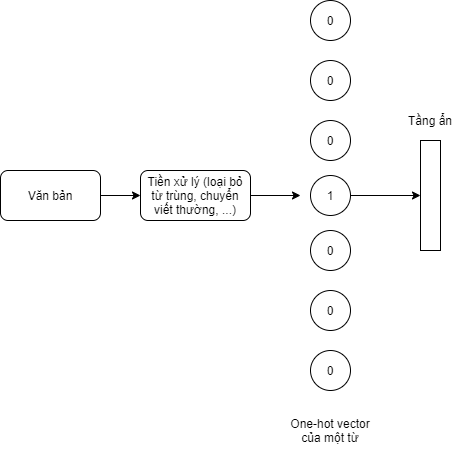
\includegraphics[scale=0.5]{02-one-hot-vector}
\caption{Ví dụ xử lý vector one-hot trong một mô hình}
\end{figure}

Tuy nhiên, việc mã hóa này không quan tâm đến ngữ nghĩa cũng như không đem lại hiệu quả tính toán, nhất là khi văn bản có số lượng lớn từ bởi nguyên nhân sẽ sinh ra một ma trận lớn nhưng thưa với đa số các phần tử bằng $0$, và chỉ số ít các phần tử có giá trị là $1$. Việc tính toán khi đưa qua các tầng cũng sẽ cho ra các vector có đa số phần tử là $0$. Để giải quyết vấn đề này, có những cách tiếp cận sau:

\subsection{Word2Vec}
Word2Vec là mô hình được đề xuất bởi Mikolov \cite{mikolov2013distributed}. Với việc lấy các one-hot vector làm đầu vào, mô hình Word2Vec tạo ra các vector có số chiều là cố định. Đồng thời các vector biểu diễn từ mang nhiều ý nghĩa hơn khi những từ mà có nghĩa gần nhau sẽ có vector gần nhau hoặc $cos$ của 2 vector lớn. Ý tưởng của mô hình này bắt nguồn từ việc con người nhận biết một từ thông qua các từ xung quanh. Ví dụ với văn bản: 

	``Hôm nay tôi đi học''
	
Khi bỏ động từ ``đi học'' để câu trở này ``Hôm nay tôi ...'', con người sẽ có khả năng đoán sau đó là một động từ. Hoặc khi giữ lại từ ``đi học'' và bỏ phần còn lại để câu trở thành ``... đi học'', người đọc cũng sẽ có xu hướng đoán trước đó phải là một danh từ ``tôi'', ``tớ'' và có thể đi kèm trước đó là trạng từ ``hôm nay'' hoặc ``hôm qua''. Từ đó, các mô hình nhúng từ về sau dựa trên ý tưởng này sẽ xem xét ngữ cảnh trong một cửa số có kích thước là $W$ để xây dựng các vector biểu diễn. 

Có $2$ mô hình tương ứng với cách dự đoán cho phần được bỏ đi như trên ví dụ đã phân tích là $CBOW\ (Continuous\  Bag\  Of\  Words)$ và $Skip-gram$. Cụ thể, $Skip-gram$ sẽ dự đoán các từ xung quanh một từ cho trước. Đầu vào của mô hình là một vector one-hot của từ đích và output là $W$ vector với $W$ là kích cỡ cửa sổ nội dung được định nghĩa với người tạo ra mô hình. Ngược lại, $CBOW$ nhận đầu vào là các $W$ từ xung quanh và cho đầu ra là vector của từ được dự đoán. 

Bằng ý tưởng trên, cùng với bộ dữ liệu 3 triệu từ cung cấp bởi Google News đã tạo ra bộ vector biểu diễn từ Word2Vec. Mỗi từ sẽ được ánh xạ đến một vector có số chiều là 300. Các vector này đã mô tả được phần nào thông tin về ngữ nghĩa. 

\subsection{fastText} 
Bộ embedding của Word2Vec dù đã nắm bắt được ngữ nghĩa của một số lượng lớn các từ, tuy nhiên vẫn tồn tại những từ không nằm trong tập từ điển. fastText ra đời và trở thành giải pháp cho vấn đề này. Đây là bộ embedding tạo ra bởi Facebook. Các vector biểu diễn từ tạo ra bởi mô hình này có thể trải qua quá trình học có giám sát hoặc không có giám sát.

Cũng giống Word2Vec, fastText sử dụng 2 mô hình là $skip-gram$ và $CBOW$. Điểm khác biệt khiến fastText có thể học được ra biểu diễn của những từ lần đầu thấy là việc mô hình này chia một từ ra thành $n$ kí tự liên tiếp nhau, hay còn gọi là n-gram mức kí tự. Một từ sẽ được thêm dấu $<$ vào đầu và $>$ vào cuối, rồi lấy ra cụm $n$ kí tự liên tiếp. Ví dụ từ ``apple'' sẽ chuyển thành ``<apple>'', lấy $n = 3$ thì được các từ con ``<ap'', ``app'', ``ppl'', ``ple'', ``le>''. Từ ``apple'' sẽ được biểu diễn dựa trên các từ con này. Việc thêm các dấu $>$ hay $<$ giúp phân biệt được từ đang xét với một từ khác. Ví dụ như biểu diễn của từ "app" là "<app>", khác với từ con "app" liệt kê phía trên được lấy ra trong từ "apple". 

\subsection{BioWordVec}
Các bộ embedding kể trên đều đã giúp biểu diễn các từ trong không gian. Tuy nhiên, để sử dụng cho từng miền dữ liệu đặc thù hơn như miền dữ liệu về Y Sinh, cần phải huấn luyện thêm bằng các tập dữ liệu thuộc miền đó. BioWordVec đã thừa kế mô hình của fastText, kết hợp với các tập dữ liệu văn bản về Y Sinh để cho ra mô hình này vào năm 2019. Cụ thể, BioWordVec cũng sử dụng tư tưởng chia một từ thành các từ con như fastText, kết hợp với tri thức miền lấy từ nguồn dữ liệu MeSH (Medical Subject Heading) hoặc hệ thống ngôn ngữ y học thống nhất (UMLS) - vốn chứa nhiều dữ liệu về Y Sinh, đã giúp nâng cao chất lượng của việc biểu diễn vector của những từ mang nhiều tính chuyên môn. 

BioWordVec cũng thừa kề ưu điểm của fastText rằng có thể tạo ra biểu diễn vector của những từ gặp lần đầu dựa trên các từ con. Điều này lại đặc biệt cần thiết trong các văn bản Y Sinh vì thường xuất hiện những từ chuyên môn như ``eltaproteobacteria''  - vốn rất hiếm gặp, và xuất hiện cũng rất thưa trong 1 văn bản. Việc chia ra thành các cụm từ quen thuộc hơn như ``bacteria'', ``delta'', ``proteo'' đã giúp tạo ra được embedding cuối cùng cho một từ hiếm, trong khi Word2Vec thì không chắc có thể cho ra biểu diễn của từ. 


\end{document}